\begin{figure}[t]
\centering
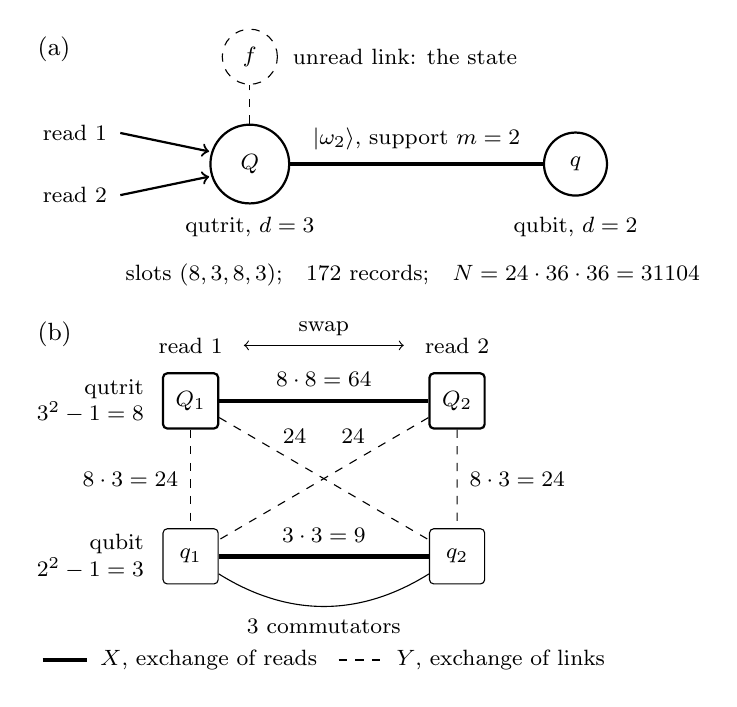
\begin{tikzpicture}[scale=0.94, every node/.style={font=\footnotesize}]
\node[draw, circle, minimum size=10mm, thick] (Q) at (0,0) {$Q$};
\node[draw, circle, minimum size=8mm, thick] (q) at (4.4,0) {$q$};
\node[draw, dashed, circle, minimum size=7mm] (f) at (0,1.45) {$f$};
\draw[very thick] (Q) -- node[above=1pt] {$|\omega_{2}\rangle$, support $m=2$} (q);
\draw[dashed] (Q) -- (f);
\node[anchor=west] at (0.45,1.45) {unread link: the state};
\node at (0,-0.85) {qutrit, $d=3$};
\node at (4.4,-0.85) {qubit, $d=2$};
\draw[->, thick] (-1.75,0.42) -- (-0.55,0.17);
\draw[->, thick] (-1.75,-0.42) -- (-0.55,-0.17);
\node[anchor=east] at (-1.8,0.42) {read 1};
\node[anchor=east] at (-1.8,-0.42) {read 2};
\node[align=center] at (2.2,-1.5) {slots $(8,3,8,3)$;\quad $172$ records;\quad $N = 24\cdot 36\cdot 36 = 31104$};
\node[anchor=north west, font=\small] at (-3.0,1.85) {(a)};
\begin{scope}[shift={(-0.8,-5.3)}, slot/.style={draw, rectangle, rounded corners=1.5pt, minimum size=7mm, inner sep=1pt}]
\node[slot, thick] (Q1) at (0,2.1) {$Q_{1}$};
\node[slot, thick] (Q2) at (3.6,2.1) {$Q_{2}$};
\node[slot] (q1) at (0,0) {$q_{1}$};
\node[slot] (q2) at (3.6,0) {$q_{2}$};
\draw[line width=1.6pt] (Q1) -- node[above=1pt] {$8\cdot 8=64$} (Q2);
\draw[line width=1.6pt] (q1) -- node[above=1pt] {$3\cdot 3=9$} (q2);
\draw[dashed] (Q1) -- node[left=1pt] {$8\cdot 3=24$} (q1);
\draw[dashed] (Q2) -- node[right=1pt] {$8\cdot 3=24$} (q2);
\draw[dashed] (Q1) -- node[pos=0.27, above right=-1pt] {$24$} (q2);
\draw[dashed] (Q2) -- node[pos=0.27, above left=-1pt] {$24$} (q1);
\draw (q1) to[bend right=32] node[below=1pt] {$3$ commutators} (q2);
\node at (0,2.85) {read 1};
\node at (3.6,2.85) {read 2};
\draw[<->] (0.72,2.85) -- node[above=0pt] {swap} (2.88,2.85);
\node[align=right, anchor=east] at (-0.5,2.1) {qutrit\\$3^{2}-1=8$};
\node[align=right, anchor=east] at (-0.5,0) {qubit\\$2^{2}-1=3$};
\draw[line width=1.6pt] (-2.0,-1.4) -- (-1.4,-1.4);
\node[anchor=west] at (-1.35,-1.4) {$X$, exchange of reads};
\draw[dashed] (2.0,-1.4) -- (2.6,-1.4);
\node[anchor=west] at (2.65,-1.4) {$Y$, exchange of links};
\end{scope}
\node[anchor=north west, font=\small] at (-3.0,-2.0) {(b)};
\end{tikzpicture}
\caption{(a)~The object: a qutrit--qubit link in the maximally entangled state $|\omega_{2}\rangle$ on its two-dimensional common support, read twice at the shared qutrit $Q$ (once on each of two links of this type, drawn as one), with a third, unread link of the same type, to the qubit $f$, carrying the state. Each read places a letter, a basis element of the traceless observables of an end, at either end of its link, its two slots, with $3^{2}-1=8$ letters at the qutrit and $2^{2}-1=3$ at the qubit, giving the slots $(8,3,8,3)$ and $172$ measurement records. The readout dimension is the traceless part of the unread link ($24 = 8\cdot 3$) times the operator space of the link at each read ($36 = 9\cdot 4$). (b)~The four slots as the corners of a square, with $Q_{1}$, $Q_{2}$ the shared qutrit's copies at the two read links and $q_{1}$, $q_{2}$ the two read qubits, each with the letters of its end. An edge is a pair of slots, not a link, and carries one product record for each letter at one end and each at the other, $64+9+4\cdot 24=169$ in all. The arc adds the $3$ commutator records, one for each pair of qubit letters, for $172$ in all. It joins the qubits only, since two reads in different bases anticommute at a qubit and no two reads anticommute at the qutrit, whose dimension is odd. Swapping the reads maps the solid edges to themselves, where $X$ acts, and the dashed edges to each other in pairs, where $Y$ acts [Eq.~(\ref{eq:s-exchanges})]; the records of the arc survive both. Tables~\ref{tab:sectors} and~\ref{tab:s-slotpairs} sort the records.}
\label{fig:link}
\end{figure}
